\chapter{Analysis of offensive capabilities} \label{chapter:analysis_offensive_capabilities}
In the previous chapter, we detailed which functionalities eBPF offers and studied its underlying architecture. As with every technology, a prior deep understanding is fundamental for discussing its security implications. 

Therefore, given the previous background, this chapter is dedicated to an analysis in detail of the security implications of a malicious use of eBPF. For this, we will firstly explore the security features incorporated in the eBPF system. Then, we will identify the fundamental pillars onto which malware can build their functionality. As we mentioned during the project goals, these main topics of research will be the following:
\begin{itemize}
\item Analysing eBPF's possibilities when hooking system calls and kernel functions.
\item Learning eBPF's potential to read/write arbitrary memory.
\item Exploring networking capabilities with eBPF packet filters.
\end{itemize}


\section{eBPF maps security}
In section \ref{subsection:access_control}, we explained that only programs with CAP\_SYS\_ADMIN are allowed to iterate over eBPF maps. The reason why this is restricted to privileged programs is because it is functionality that is a potential security vulnerability, which we will now proceed to analyse.

Also, in section \ref{subsection:ebpf_maps}, we mentioned that eBPF maps are opened by specifying an ID (which works similarly to the typical file descriptors), while in table \ref{table:ebpf_map_types} we showed that, for performing operations over eBPF maps using the bpf() syscall, the map ID must be specified too. 

Map IDs are known by a program after creating the eBPF map, however, a program can also explore all the available maps in the system by using the BPF\_MAP\_GET\_NEXT\_ID operation in the bpf() syscall, which allows for iterating through a complete hidden list of all the maps created. This means that privileged programs can find and have read and write access to any eBPF map used by any program in the system.

Therefore, a malicious privileged eBPF program can access and modify other programs' maps, which can lead to:
\begin{itemize}
\item Modify data used for the program operation. This is the case for maps which mainly store data structures, such as BPF\_MAP\_TYPE\_HASH.
\item Modify the program control flow, altering the instructions executed by an eBPF program. This can be achieved if a program is using the bpf\_tail\_call() helper (introduced in table \ref{table:ebpf_helpers}) which is taking data from a map storing eBPF programs (BPF\_MAP\_TYPE\_PROG\_ARRAY, introduced in table \ref{table:ebpf_map_types}).
\end{itemize}


\section{Abusing tracing programs}
eBPF tracing programs (kprobes, uprobes and tracepoints) are hooked to specific points in the kernel or in the user space, and call probe functions once the flow of execution reaches the instruction to which they are attached. This section details the main security concerns regarding this type of programs.

\subsection{Access to function arguments} \label{subsection:tracing_arguments}
As we saw in section \ref{section:ebpf_prog_types}, tracing programs receive as a parameter those arguments with which the hooked function originally was called. These parameters are read-only and thus, in principle, they cannot be modified inside the tracing program (we will show this is not entirely true in section \ref{section:mem_corruption}). The next code snippets show the format in which parameters are received when using libbpf (Note that libbpf also includes some macros that offer an alternative format, but the parameters are the same).

\begin{lstlisting}[language=C, caption={Probe function for a kprobe on the kernel function vfs\_write.}, label={code:format_kprobe}]
SEC("kprobe/vfs_write")
int kprobe_vfs_write(struct pt_regs* ctx){
\end{lstlisting}

\begin{lstlisting}[language=C, caption={Probe function for an uprobe, execute\_command is defined from user space.}, label={code:format_uprobe}]
SEC("uprobe/execute_command")
int uprobe_execute_command(struct pt_regs *ctx){
\end{lstlisting}

\begin{lstlisting}[language=C, caption={Probe function for a tracepoint on the start of the syscall sys\_read.}, label={code:format_tracepoint}]
SEC("tp/syscalls/sys_enter_read") 
int tp_sys_enter_read(struct sys_read_enter_ctx *ctx) { 
\end{lstlisting}

In code snippets \ref{code:format_kprobe} and \ref{code:format_uprobe} we can identify that the parameters are passed to kprobe and uprobe programs as a pointer to a \textit{struct pt\_regs*}. This struct contains as many attributes as registers exist in the system architecture, in our case x86\_64. Therefore, on each probe function, we will receive the state of the registers at the original hooked function. This explains the format of the \textit{struct pt\_regs}, shown in code snippet \ref{code:format_ptregs}:

\begin{lstlisting}[language=C, caption={Format of struct pt\_regs.}, label={code:format_ptregs}]
struct pt_regs {
	long unsigned int r15;
	long unsigned int r14;
	long unsigned int r13;
	long unsigned int r12;
	long unsigned int bp;
	long unsigned int bx;
	long unsigned int r11;
	long unsigned int r10;
	long unsigned int r9;
	long unsigned int r8;
	long unsigned int ax;
	long unsigned int cx;
	long unsigned int dx;
	long unsigned int si;
	long unsigned int di;
	long unsigned int orig_ax;
	long unsigned int ip;
	long unsigned int cs;
	long unsigned int flags;
	long unsigned int sp;
	long unsigned int ss;
};
\end{lstlisting}

By observing the value of the registers, we can extract the parameters of the original hooked function. This can be done by using the System V AMD64 ABI\cite{8664_params_abi}, the calling convention used in Linux. Depending on whether we are in the kernel or in user space, the registers used to store the values of the function arguments are different. Table \ref{table:systemv_abi} summarizes these two interfaces. 

\begin{table}[H]
\begin{tabular}{|>{\centering\arraybackslash}p{2cm}|>{\centering\arraybackslash}p{3cm}|}
\hline
\multicolumn{2}{|c|}{User interface}\\
\hline
Register & Purpose\\
\hline
\hline
rdi & 1st argument\\
\hline
rsi & 2nd argument\\
\hline
rdx & 3rd argument\\
\hline
rcx & 4th argument\\
\hline
r8 & 5th argument\\
\hline
r9 & 6th argument\\
\hline
rax & Return value\\
\hline
\end{tabular}
\quad
\begin{tabular}{|>{\centering\arraybackslash}p{2cm}|>{\centering\arraybackslash}p{3cm}|}
\hline
\multicolumn{2}{|c|}{Kernel interface}\\
\hline
Register & Purpose\\
\hline
\hline
rdi & 1st argument\\
\hline
rsi & 2nd argument\\
\hline
rdx & 3rd argument\\
\hline
r10 & 4th argument\\
\hline
r8 & 5th argument\\
\hline
r9 & 6th argument\\
\hline
rax & Return value\\
\hline
\end{tabular}
\caption{Argument passing convention of registers for function calls in user and kernel space respectively.}
\label{table:systemv_abi}
\end{table}

In the case of tracepoints, we can see in code snippet \ref{code:format_tracepoint} that it receives a \textit{struct sys\_read\_enter\_ctx*}. This struct must be manually defined, as explained in \ref{subsection:tracepoints}, by looking at the file \textit{/sys/kernel/debug/tracing/events/syscalls/sys\_enter\_read/format}. Code snippet \ref{code:sys_enter_read_tp} shows the format of the struct.

\begin{lstlisting}[language=C, caption={Format for parameters in sys\_enter\_read specified at the format file.}, label={code:sys_enter_read_tp_format}]
field:unsigned short common_type; offset:0; size:2; signed:0;
field:unsigned char common_flags; offset:2; size:1; signed:0;
field:unsigned char common_preempt_count; offset:3; size:1; signed:0;
field:int common_pid; offset:4; size:4; signed:1;
field:int __syscall_nr;	offset:8; size:4; signed:1;
field:unsigned int fd; offset:16; size:8; signed:0;
field:char * buf; offset:24; size:8; signed:0;
field:size_t count; offset:32; size:8; signed:0;
\end{lstlisting}

\begin{lstlisting}[language=C, caption={Format of custom struct sys\_read\_enter\_ctx.}, label={code:sys_enter_read_tp}]
struct sys_read_enter_ctx {
    unsigned long long pt_regs;
    int __syscall_nr;
    unsigned int padding;
    unsigned long fd;
    char* buf;
    size_t count;
};
\end{lstlisting}

As we can observe, we are given a set of attributes which include the parameters with which the syscall was called. Moreover, we can still obtain an address pointing to another \textit{struct pt\_regs}, as in kprobes and uprobes, by combining the first four fields and considering it as a 32-bit long address. This means we will still be able to extract the value of the rest of the registers too. 

It must be noted that, in syscalls, in addition to use the kernel parameter passing convention specified in table \ref{table:systemv_abi}, the number specifying the syscall must be passed in register rax too.

On a final note, as we mentioned in section \ref{section:ebpf_prog_types}, there exist differences in the parameters received in probe functions depending on the two variations of tracing programs. Therefore:
\begin{itemize}
\item kprobe, uprobe and \textit{enter} tracepoints will receive the full parameters as we specified before, but not the return value of the function (since it is not executed yet).
\item kretprobes, uretprobes and \textit{exit} tracepoints will still receive the \textit{struct pt\_regs}, but without any of the parameters and with only the return value of the function.
\end{itemize}

Taking into account all the previous, the fact that tracing programs have read-only access to function arguments can be considered a useful and needed feature for tracing applications, but malicious eBPF can use this for purposes such as:
\begin{itemize}
\item Gather kernel and user data passed to a function as a parameter. In many cases this information can be potentially interesting for an attacker, such as passwords.
\item Store in eBPF maps information about system activities, to be used by other malicious eBPF programs.
\end{itemize}

Usually, since many function arguments are pointers to user or kernel addresses (such as buffers where a string or a struct with data is located), eBPF tracing programs can use two eBPF helpers that enable to read large byte arrays from both kernel and user space:
\begin{itemize}
\item bpf\_probe\_read\_user()
\item bpf\_probe\_read\_kernel()
\end{itemize}

These helpers, previously introduced in table \ref{table:ebpf_helpers}, enable to read an arbitrary number of bytes from an user or kernel address respectively, allowing us to extract the information pointed by the parameters received by eBPF programs.

\subsection{Reading memory out of bounds} \label{subsection:out_read_bounds}
As we introduced in the previous subsection, the bpf\_probe\_read\_user() and bpf\_probe\_read\_kernel() helpers can be used to access memory of pointers received as parameters in the hooked functions. 

However, although in general the eBPF verifier attempts to reject illegal memory accesses, it does not prevent a malicious program from passing an arbitrary memory address (in kernel or user space) to the above helpers. This means that an eBPF program can potentially read any address in user or kernel space, (as long as it is marked as readable in the corresponding memory pages). Furthermore, an attacker can locate specific data structures and memory sections by taking the function parameter as a reference point in memory.

A particularly relevant case (which we will later use for our rootkit) involves accessing user memory via the parameters of tracepoints attached at system calls. Provided the nature of syscalls, whose purpose is to communicate user and kernel space, all parameters received will belong to the user space, and therefore any pointer passed will be an address in user memory. This enables an eBPF program to get a foothold into the virtual address space of the process calling the syscall, which it can proceed to scan looking for data or specific instructions. This technique will be further elaborated in section \ref{subsection_bpf_probe_write_apps}.

\subsection{Overriding function return values}
A potentially dangerous functionality in eBPF tracing programs is the ability to modify the return value of kernel functions\cite{ebpf_friends_p15}\cite{ebpf_override_return}. This can be done via the eBPF helper bpf\_override\_return, and it works exclusively from kretprobes.

Apart from only working on kretprobes, additional restrictions are applied to this helper. It will only work if the kernel was compiled with the CONFIG\_BPF\_KPROBE\_OVERRIDE flag, and only if the kretprobe is attached to a function to which, during the kernel development, the macro ALLOW\_ERROR\_INJECTION() has been indicated. Currently, only a small selection of functions includes this macro, but most system calls can be found to implement it. The following code snippets show how a system call like sys\_open is defined in kernel v5.11:

\begin{lstlisting}[language=C, caption={Definition of the syscall sys\_open in the kernel \cite{code_kernel_open}}, label={code:override_return_1}]
SYSCALL_DEFINE3(open, const char __user *, filename, int, flags, umode_t, mode)
{
	if (force_o_largefile())
		flags |= O_LARGEFILE;
	return do_sys_open(AT_FDCWD, filename, flags, mode);
}
\end{lstlisting}

\begin{lstlisting}[language=C, caption={Definition of the macro for creating syscalls, containing the error injection macro. Only relevant instructions included, complete macro can be found in the kernel \cite{code_kernel_syscall}}, label={code:override_return_2}]
#define SYSCALL_DEFINE3(name, ...) SYSCALL_DEFINEx(3, _##name, __VA_ARGS__)
#ifndef __SYSCALL_DEFINEx
#define __SYSCALL_DEFINEx(x, name, ...)\
	[...]
	ALLOW_ERROR_INJECTION(sys##name, ERRNO);\
	[...]
\end{lstlisting}


By looking at snippets \ref{code:override_return_1} and \ref{code:override_return_2}, we can observe that the system call sys\_open involves the inclusion of the ALLOW\_ERROR\_INJECTION macro. Therefore, any kretprobe attached to a system call function will be able to modify its return value.

In order to be able to modify the return value of functions, the aforementioned eBPF helper makes use of the fault injection framework of the Linux kernel\cite{fault_injection}, which was created before eBPF itself, and whose original purpose is to allow for generating errors in kernel programs for debugging purposes.

Taking the previous information into account, we can find that a malicious eBPF program, by tampering with the kernel-user space interface which are system calls, can mislead user programs, which trust the output of kernel code. This can lead to:
\begin{itemize}
\item A program believes a system call exited with an error, while in reality the kernel completed the operation with success, or vice versa. For instance, the result of a call to sys\_open can mislead a user program into thinking that a file does not exist.
\item A program receives incorrect data on purpose. For instance, a buffer may look empty or of a reduced size upon a sys\_read call, while in reality more data is available to be read.
\end{itemize}

\subsection{Sending signals to user programs}
Another eBPF helper that is subject to malicious purposes is bpf\_send\_signal. This helper enables to send an arbitrary signal to the thread of the process running a hooked function.

Therefore, this helper can be used to forcefully terminate running user processes, by sending the SIGKILL signal. In this way, combined with the observability into the parameters received at a function call, malicious eBPF can kill and deactivate processes to favour its malicious purposes.

\subsection{Takeaways} \label{subsection:tracing_attacks_conclusion}
As a summary, a malicious eBPF program loaded and attached as a tracing program undermines the existing trust between user programs and the kernel space. 

Its ability to access sensitive data in function parameters and reading arbitrary memory can lead to gathering extensive information on the running processes of a system, whilst the malicious use of eBPF helpers enables the modification of the data passed to the user space from the kernel, and the control over which programs are allowed to be running on the system.

\section{Memory corruption} \label{section:mem_corruption}
In the previous section we described how tracing programs can read user memory out of the bounds of function parameters via the helpers bpf\_probe\_read\_user() and bpf\_probe\_read\_kernel(). In this section, we will analyse another eBPF helper can be found to be the heart of malicious programs.

Privileged eBPF programs (or those with at least CAP\_BPF + CAP\_PERFMON capabilities) have the potential to use an experimental (it is labelled as so \cite{ebpf_helpers}) helper called bpf\_probe\_write\_user(). This helper enables to write into user memory from within an eBPF program. 

However, this helper has certain limitations that restrict its use. We will now proceed to review some background into how user memory works and, afterwards, we will analyse the restrictions and possible uses of this eBPF helper in the context of malicious applications.


\subsection{Attacks and limitations of bpf\_probe\_write\_user()} \label{subsection:bpf_probe_write_apps}
Provided the background into memory architecture and the stack operation, we will now study the offensive capabilities of the bpf\_probe\_write\_user() helper and which restrictions are imposed into its use by eBPF programs.

The bpf\_probe\_write\_user() helper, when used from a tracing eBPF program, can write into any memory address in the user space of the process responsible from calling the hooked function. However, the write operation fails has some restrictions:
\begin{itemize}
\item{The operation fails if the memory space pointed by the address is marked as non-writeable by the user space process. For instance, if we try to write into the .text section, the helpers fails because this section is only marked as readable and executable (for protection reasons).} Therefore, the process must indicate a writeable flag in the memory section for the helper to succeed.
\item{The operation fails if the memory page is served with a minor or major page fault \cite{bpf_probe_write_user_errors}. As we saw in section \ref{subsection:ebpf_verifier}, eBPF programs are restricted from executing any sleeping or blocking operations, to prevent hanging the kernel. Therefore, since during a page fault the operating system needs to block the execution and write into the page table or retrieve data from the secondary disk, bpf\_probe\_write\_user() is defined as a non-faulting helper\cite{write_helper_non_fault}, meaning that instead of issuing a page fault for accessing data, it will just return and fail.}
\item{Each time the helper is called, an alert message is written into the kernel logs, alerting that a potentially dangerous eBPF program is making use of the helper. Note that this message appears when the eBPF program is attached, and not each time the helper is called. This will be particularly relevant since we will be able to bypass this alert by taking advantage of this.}
\end{itemize}

Although we will not be able to modify kernel memory or the instructions of a program, this eBPF helper opens a range of possible attacks:
\begin{itemize}
\item Modify any of the arguments with which a system call is called (either with a tracepoint or a kprobe). Therefore, a malicious program can hijack any call to the kernel with its own arguments.
\item Modify user-provided arguments in kernel functions. When reading kernel code, we can find that data provided by the user is marked with the keyword \textit{\_\_user}. For instance, an internal kernel function in a nested call of the system call sys\_read receives an user buffer:
\begin{lstlisting}[language=C, caption={Definition of kernel function vfs\_read. \cite{code_vfs_read}}, label={code:vfs_read}]
ssize_t vfs_read(struct file *file, char __user *buf, size_t count, loff_t *pos)
\end{lstlisting}
Then, if we attach a kprobe to vfs\_read, we would be able to modify the value of the buffer.
\item Modify process memory by taking function parameters as a reference and scanning the stack. This technique, first introduced in section \ref{subsection:out_read_bounds} when we mentioned that tracing programs can read any user memory location with the bpf\_probe\_read\_user() helper, and which was publicly first used by Jeff Dileo at his talk in DEFCON 27\cite{evil_ebpf_p6974}, consists of:
\begin{enumerate}
\item Take an user-passed parameter received on a tracing program. The parameter must be a pointer to a memory location (such as a pointer to a buffer), so that we can use that memory address as the reference point in user space. According to the x86\_64 documentation, this parameter will be stored in the stack\cite{8664_params_abi_p1922}, so we will receive a stack address.
\item Locate the target data which we aim to write. There are two main methods for this:
\begin{itemize}
	\item Sequentially read the stack, using bpf\_probe\_read\_user(), until we locate the bytes we are looking for. This requires knowing which data we want to overwrite.
	\item By previously reverse engineering the user program, we can calculate the offset at which an specific data section will be stored in virtual memory with respect to the reference address we received as a parameter.
\end{itemize}
\item Overwrite the memory buffer using bpf\_probe\_write\_user().
\end{enumerate}
\end{itemize}

Figure \ref{fig:stack_scan_write_tech} illustrates a high-level overview of the stack scanning technique previously described.
%TODO i just noticed I included SFP outside the current stack frame, correct it here and everywhere
\begin{figure}[H]
	\centering
	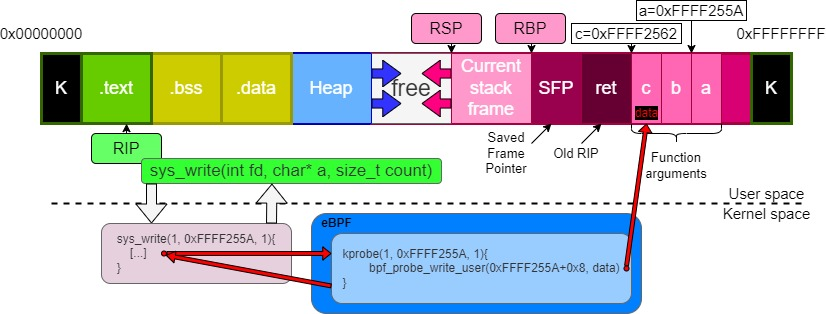
\includegraphics[width=16cm]{stack_scan_write_tech.jpg}
	\caption{Overview of stack scanning and writing technique.}
	\label{fig:stack_scan_write_tech}
\end{figure}

The figure shows process memory executing a program similar to the following:
\begin{lstlisting}[language=C, caption={Sample program being executed on figure \ref{fig:stack_scan_write_tech}.}, label={code:stack_scan_write_tech}]
void func(char* a, char* b, char* c){
	int fd = open("FILE", 0);
	write(fd, a, 1);
}

int main(){
	char a[] = "AAA";
	char b[] = "BBB";
	char c[] = "CCC";
	func(a, b, c);
}
\end{lstlisting}

In the figure, we can clearly observe how the technique is used to overwrite a specific buffer. The attacker goal is to overwrite buffer \textit{c} with some other bytes, but the kprobe program only has direct access to buffer \textit{a}:
\begin{enumerate}
\item By reverse engineering the program (we will see how this process works in section \ref{TODO}) we notice that buffer \textit{c} is stored 8 bytes lower on the stack than buffer \textit{a}.
\item When register rip points to the write() instruction, the processor executes the instruction and a system call is issued to sys\_write().
\item The kprobe eBPF program hooked to the syscall hijacks the program execution. Since it has access to the memory address of buffer \textit{a} and it knows the relative position of buffer \textit{c}, it writes to that location whatever it wants (e.g.: "DDD") with the bpf\_probe\_write\_user() helper.
\item The eBPF program ends and the control flow goes back to the system call. It ends its execution successfully and returns a value to the user space. The result of the program is that 1 byte has been written into file "FILE", and that buffer \textit{c} now contains "DDD".
\end{enumerate}

\subsection{Takeaways}
As a summary, the bpf\_probe\_write\_user() helper is one of the main attack vectors for malicious eBPF programs. Although it does contain some restrictions, its ability to overwrite any user parameter enables it to, in practice, execute arbitrary code by hijacking that of others. When it is combined with tracing programs' ability to read memory out of bounds, it unlocks a wide range of attacks, since any writeable section of the process memory is a possible target. 

Therefore, if on the conclusion of section \ref{subsection:tracing_attacks_conclusion} we discussed that the ability to change the return value of kernel functions and kill processes hinders the trust between the user and kernel space (since what the kernel returns may not be a correct result), then the ability to directly overwrite process data is a complete disrupt of trust in any of the data in the user space itself, since it is subject to the control of a malicious eBPF program.

Moreover, in the next sections we will discuss how we can create advanced attacks based on the background and techniques previously discussed. We will research further into which sections of a process memory are writeable and whether they can lead to new attack vectors.


\section{Abusing networking programs}\label{section:abusing_networking}
The final main piece of a malicious eBPF program comes from taking advantage of the networking capabilities of TC and XDP programs. As we mentioned during sections \ref{subsection:xdp} and \ref{subsection:tc}, these type of programs have access to network traffic:
\begin{itemize}
\item Traffic Control programs can be placed either on egress or ingress traffic, and receive a struct \textit{sk\_buff}, containing the packet bytes and meta data that helps operating on it.
\item External Data Path programs can only be attached to ingress traffic, but in turn they receive the packet before any kernel processing (as a struct \textit{xdp\_md}) being able to access the raw data directly.
\end{itemize}

Networking eBPF programs not only have read access to the network packets, but also write access:
\begin{itemize}
\item XDP programs can directly modify the raw packet via memcpy() operations. They can also increment or reduce the size of the packet at any of its ends (adding bytes before the head or after the packet tail). This is done via the multiple helpers previously presented on table \ref{table:xdp_helpers}.
\item TC programs can also modify the packet via the helpers presented on table \ref{table:tc_helpers}. The packet can be expanded or reduced via these eBPF helpers too.
\end{itemize} 

Apart from write access to the packet, the other critical feature of networking programs is their ability to drop packets. As we presented in tables \ref{table:xdp_actions_av} and \ref{table:tc_actions}, this can be achieved by returning specific values.


\subsection{Attacks and limitations of networking programs} \label{subsection:network_attacks}
Based on the previous background, we will now proceed to explore which limitations exist on which actions a network eBPF program can perform:
\begin{itemize}
\item Read and write access to the packet is heavily controlled by the eBPF verifier. It is not possible to read or write data out of bounds. Extreme care must also be taken before attempting to read any data inside the packet, since the verifier first requires making lots of checks beforehand. For any access to take place, the program must first classify the packet according to the network protocol it belongs, and later check that every header of every layer is well defined (e.g.: Ethernet, IP and TCP). Only after that, the headers can be modified. 

If the program also wants to modify the packet payload, then it must be checked to be between the bounds of the packet and well defined according to the packet headers(using fields IHL, packet length and data offset, in figure \ref{fig:frame}). Also, after using any of the helpers that enlarge or reduce the size of the packet, all check operations must be repeated before any subsequent operation.

Finally, note that after any modification in the packet, some network protocols (such as IP and TCP) require to recalculate their checksum fields. 

\item XDP and TC programs are not able to create packets, they can only operate over existing traffic.

\item If an XDP program modifies an incoming packet, the kernel will not know about the original data, but if an egress TC program modifies a packet being sent, the kernel will be able to notice the modification.
\end{itemize}

Having the previous restrictions in mind, we can find multiple possible malicious uses of an XDP/TC program:
\begin{itemize}
\item \textbf{Spy all network connections} in the system. An XDP or TC ingress program can read any packet from any interface, therefore achieving a comprehensive view on which are the running communications and opened ports (even if protocols with encryption are being used) and gathering transmitted data (if the connection is also in plaintext).
\item \textbf{Hide arbitrary traffic} from the host. If an XDP program drops a packet, the kernel will not be able to know any packet was received in the first place. This can be used to hide malicious incoming traffic. However, as we will mention in section \ref{section:c2}, malicious traffic may still be detected by other external devices, such as network-wide firewalls.
\item \textbf{Modify incoming traffic} with XDP programs. Every packet can be modified (as we mentioned at the beginning of section \ref{section:abusing_networking}), and any modification will be unnoticeable to the kernel, meaning that we will have complete, invisible control over the packets received by the kernel.
\item \textbf{Modify outgoing traffic} with TC egress programs. Since every packet can be modified at will, we will therefore have complete control over any packet sent by the host. This can be used to enable a malicious program to communicate over the network and exfiltrate data, since even if we cannot create a new connection from eBPF, we can still modify existing packets, writing any payload and headers on it (thus being able to, for instance, change the destination of the packet).

Notice, however, that these modifications are not transparent to the kernel as with XDP, and thus an internal firewall may detect our malicious traffic.
\end{itemize}

Although we mention the possibility of modifying outgoing traffic as an alternative to the impossibility of sending new packets from eBPF, there exists a major disadvantage by doing this, since the original packet of the application will be lost, and we will thus be disrupting the normal functioning of the system (which in a rootkit is unacceptable, as we mentioned in section \ref{section:motivation}, stealth is a priority).

There exists, however, a simple way of duplicating a packet so that the original packet is not lost but we can still send our overwritten packet. This technique, first presented by Guillaume Fournier and Sylvain Afchainthe in their DEFCON talk, consists of taking advantage of TCP retransmissions we described on section \ref{subsection:tcp}. Figure \ref{fig:tcp_exfiltrate_retrans} shows this process:

\begin{figure}[H]
	\centering
	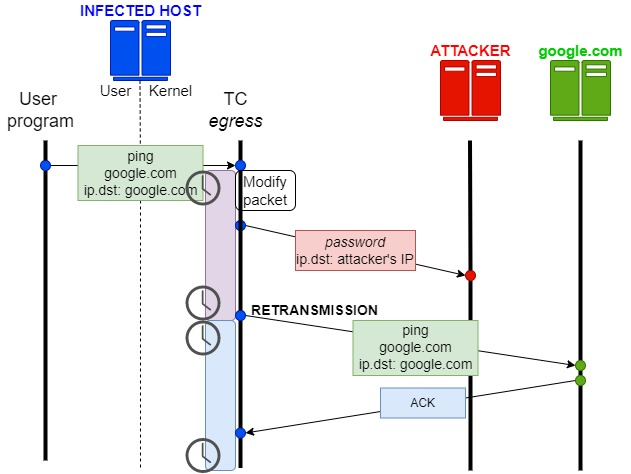
\includegraphics[width=15cm]{tcp_exfiltrate_retrans.jpg}
	\caption{Technique to duplicate a packet for exfiltrating data.}
	\label{fig:tcp_exfiltrate_retrans}
\end{figure}

In the figure, we can observe a host infected by a malicious TC egress program. An user space application at some point needs to send a packet (in this case a simple ping), and the TC program will overwrite it (in this case, it writes a password which it has been able to find, and substitutes the destination IP address with that of a listening attacker.
After the timer runs out, the TCP protocol itself will retransmit the same packet as previously and thus the original data is delivered too.

Using this technique, we will be able to send our own packets every time an application sends outgoing traffic. And, unless the network is being monitored, this attack will go unnoticed, provided that the delay of the original packet is similar to that when a single packet lost.

\subsection{Takeaways}
As a summary, networking eBPF programs offer complete control over incoming and outgoing traffic. If tracing programs and memory corruption techniques served to disrupt the trust in the execution of both any user and kernel program, then a malicious networking program has the potential to do the same with any communication, since any packet is under the control of eBPF.

Ultimately, the capabilities discussed in this section unlock complete freedom for the design of malicious programs. As we will explain in the next chapter, one particularly relevant type of application can be built:
\begin{itemize}
\item A \textbf{backdoor}, a stealthy program which listens on the network interface and waits for secret instructions from a remote attacker-controlled client program. This backdoor can have \textbf{Command and Control (C2)} capabilities, meaning that it can process commands sent by the attacker and received at the backdoor, executing a series of actions corresponding to the request received, and (when needed) answering the attacker with the result of the command.
\end{itemize}

%TODO maybe a conclusion for this chapter?
